\documentclass[UTF8,a4paper,zihao=5,fontset=fandol]{ctexart}
\usepackage[margin=21mm,top=19mm,bottom=19mm]{geometry}
\usepackage{amsmath,amssymb,graphicx,booktabs,array,caption,xcolor,adjustbox}
\usepackage[hidelinks]{hyperref}
\usepackage{fancyhdr}
\pagestyle{fancy}\fancyhf{}\fancyhead[L]{\small 机器学习课程设计}\fancyhead[R]{\small 二维变分网格与步长预测}
\fancyfoot[C]{\thepage}\setlength{\headheight}{15pt}
\setlength{\parskip}{3pt}\linespread{1.12}
\ctexset{section={format=\large\bfseries,beforeskip=8pt,afterskip=4pt},subsection={format=\normalsize\bfseries,beforeskip=6pt,afterskip=3pt}}
\captionsetup{font=small,labelformat=empty,hypcap=false,skip=3pt}
\setlength{\emergencystretch}{1em}
\begin{document}
\begin{center}{\LARGE\bfseries 机器学习辅助的二维变分移动网格优化}\end{center}

基于初始步长预测的数值实验


作者：\_\_\_\_\_\_\_\_　学号：\_\_\_\_\_\_\_\_　课程：机器学习课程设计


\textbf{摘要：} 针对二维变分网格梯度优化中的步长选择问题，本文复用 Winslow 离散能量、解析梯度与逆映射，构建带合法性和 Armijo 充分下降检查的随机森林步长预测方法。采用完整网格实例划分，利用传统线搜索轨迹训练模型，并在均匀、高斯及各向异性三类度量下，与固定步长、标准 Armijo 和热启动策略比较。九个未见实例的三十六次运行均达到相同相对梯度阈值，最终网格无翻转。学习方法虽减少部分能量评价，推理开销却使总耗时高于传统方法。结果说明评价次数减少并不等于实际加速，小型网格应优先采用低开销步长策略。


\textbf{关键词：} 变分网格；随机森林；Armijo 线搜索；步长预测；数值实验


\section*{1 引言}

移动网格在保持节点数量和连接关系的条件下调整节点位置，使计算资源向局部变化较强的区域集中。变分方法通过最小化网格泛函确定坐标映射；不同泛函对网格的集中、形状与边界约束有不同响应[1]。本文关注其中一个有限而明确的问题：在能量和下降方向固定时，能否利用机器学习选择更合适的线搜索初始步长？


学习线搜索已有相关研究。Kamandi 使用循环模型预测步长和退缩因子[2]；Wu 等将回归模型用于变分网格中的流场估计[3]。本文仅使用一个随机森林预测初始步长，通过小规模对照实验检验其必要性和实际成本。实验复用本地已有数值模块，所有图表均由保存的数值轨迹生成。


\section*{2 方法}

\subsection*{2.1 离散能量与坐标角色}

设固定物理顶点为 $X$，计算顶点为 $Q$，参考顶点为 $\widehat Q$。单元边矩阵分别为 $E_K=[x_1-x_0,x_2-x_0]$ 和 $B_K=[q_1-q_0,q_2-q_0]$，令 $J_K=B_KE_K^{-1}$。固定物理单元面积和单元中心度量后，使用


\[
I_h(Q)=\sum_K |K|\,\operatorname{tr}(J_K M_K^{-1}J_K^T).
\]

该能量对应[1]式(6)的离散形式，省略了常数因子 $1/2$，梯度与步长均按本实现定义。令 $C_K=E_K^{-1}M_K^{-1}E_K^{-T}$，则单元对边矩阵的导数为 $2|K|B_KC_K$；两列分别装配到顶点1和2，负的列和装配到顶点0。固定边界节点的梯度投影为零。计算过程中 $X$、$|K|$ 和 $M_K$ 不变，最终物理网格由分片线性映射 $\Phi_h:Q\mapsto X$ 在 $\widehat Q$ 上求值得到。


\newpage

\subsection*{2.2 共同的下降与合法性条件}

记投影梯度为 $g_k$。四种方法均沿 $-g_k$ 更新计算坐标，候选步为 $Q_k-\alpha g_k$。Armijo 条件为


\[
I_h(Q_k-\alpha g_k)\le I_h(Q_k)-c_1\alpha\|g_k\|_2^2,\qquad c_1=10^{-4}.
\]

首先检查候选计算网格的定向面积，再计算候选能量和梯度；充分下降满足后重建物理网格，检查所有物理三角形的定向面积。两类面积均须大于 $10^{-12}$。线搜索失败时，Armijo、热启动和随机森林方法以 $\beta=1/2$ 退缩；随机森林搜索耗尽可回退到默认初值。固定步长为0.05，不作回溯，若不能满足同样的接受条件则终止并记录失败。


停止条件统一为


\[
\|g_k\|_2\le\max(10^{-7},10^{-4}\|g_0\|_2).
\]

每次运行最多1800次接受迭代、30000次能量评价；每轮回溯最多40次。计算网格边界始终固定，重建物理网格边界位移仅有插值舍入误差。记录成功和失败运行，比较采用相同网格、相同精度和相同预算。


\subsection*{2.3 随机森林和数据划分}

以标准 Armijo 接受的 $\log\alpha_k$ 为监督标签。四个可用特征为


\[
z_k=\left[\log(1+\|g_k\|_2),\ \log\alpha_{k-1},\ \log(2n^2 A_{\min,k}),\ b_{k-1}\right].
\]

其中 $A_{\min,k}$ 为当前计算网格最小定向面积，$b_{k-1}$ 为上一步拒绝候选数，初值为 $\alpha_{-1}=1$、$b_{-1}=0$。森林含32棵树，最大深度10，叶节点最少5个样本，固定随机种子20261020，单线程预测。预测值经指数和裁剪得到 $\alpha_0=\operatorname{clip}(\exp f(z_k),10^{-12},1)$。


训练集为每类8个实例，共24条完整轨迹；验证集为每类2个，共6个实例；测试集为每类3个，共9个实例。训练、验证和测试种子分别为0–7、80–81、100–102。训练和验证网格取 $n\in\{8,10,12\}$，测试统一 $n=12$。模型使用 4620 个训练步骤和 1172 个验证步骤；同一实例的全部步骤仅属于一个集合。超参数固定，不根据测试结果选择。


算法流程：生成传统轨迹 $\to$ 按实例分组 $\to$ 训练森林 $\to$ 读取当前状态并预测初值 $\to$ 检查计算网格 $\to$ 检查充分下降 $\to$ 重建并检查物理网格 $\to$ 接受或回溯 $\to$ 记录日志。


\subsection*{2.4 基本数学核验}

原模块的单元手算能量、解析梯度方向差分、恒等重建及能量与正面积测试共5项通过。本项目再对三类度量各取两个随机合法网格进行中心差分，步幅 $10^{-5}$，最大相对误差为 6.45e-09，并检查负梯度小步下降。每个接受步执行下降、有限值和边界检查；数据划分执行实例集合不相交断言。


\newpage

\section*{3 数值实验}

\subsection*{3.1 环境、参数与计时口径}

实验在本地 Windows 环境运行，Python 3.13.2、NumPy 2.3.4、scikit-learn 1.9.1，使用CPU。完整依赖版本保存于环境记录。几何与优化为 NumPy 运算，森林使用 scikit-learn，不依赖GPU或完整PDE系统。


区域为单位正方形，先将每个方格剖分成两个正定向三角形，得到 $n=12$ 时169个顶点和288个单元。每个内部物理顶点的两个坐标独立均匀扰动，范围为 $[-0.12/n,0.12/n]$；边界不动。计算初值为规则参考网格。同一实例四种方法使用完全一致的输入。按种子轮换运行顺序，减轻固定顺序影响。


表1　三类算例的共同构造


\begin{center}\small\begin{adjustbox}{max width=\linewidth}\begin{tabular}{lll}\toprule
算例 & 单元中心度量 & 目的 \\
\midrule
均匀 & $M=I$ & 扰动平滑与稳定性 \\
高斯 & $M=(1+w)I$ & 局部节点集中 \\
各向异性 & $M=I+wvv^T$ & 定向变形 \\
\bottomrule\end{tabular}\end{adjustbox}\end{center}

这里 $w=s\exp(-\|x-c\|^2/(2\sigma^2))$，$\sigma=0.17$，$s$ 在[3,7]中采样，中心两个坐标在[0.43,0.57]中采样，$v=(\cos(\pi/6),\sin(\pi/6))^T$。高斯度量特征值均为 $1+w$，各向异性度量特征值为1和 $1+w$，因而所有输入度量均正定。具体参数逐实例保存在配置文件中。


总耗时覆盖能量对象初始化、特征提取、模型推理、候选检查、梯度计算、网格重建及相同的历史记录工作；不包含实例生成、文件写入和训练。能量评价计数包含初始能量，每次调用复用接口同时获得能量与梯度，拒绝候选的梯度也计入成本。面积检查拒绝的候选不计能量评价；回溯数统计被拒绝的候选，因此二者不能简单互换。搜索耗时包含网格重建，不等同于重复能量评价的纯成本。


\subsection*{3.2 算例一：均匀度量}

\begin{center}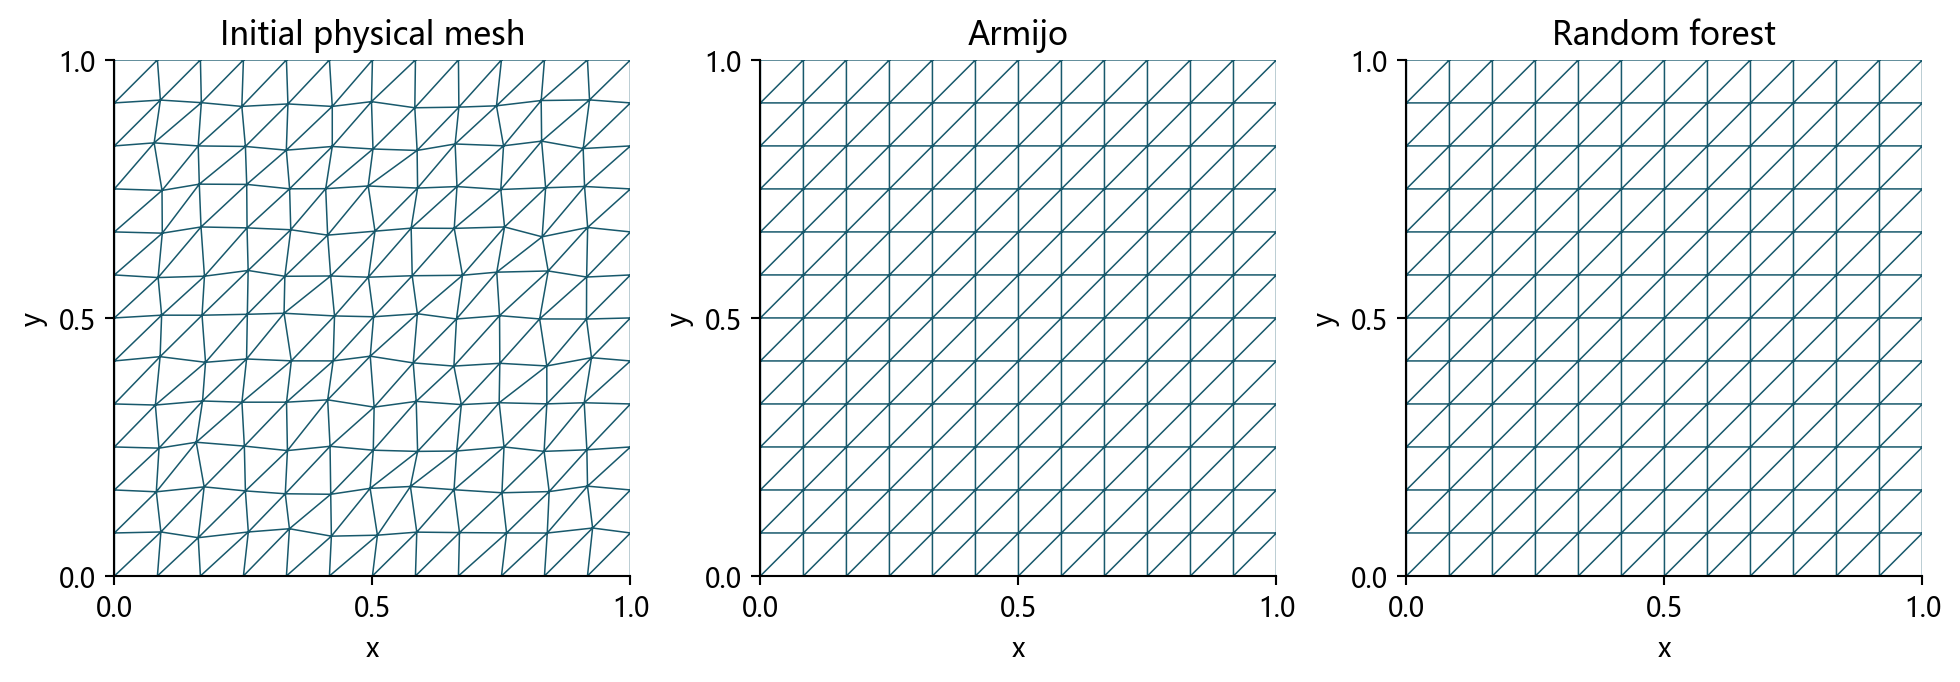
\includegraphics[width=\linewidth]{../figures/mesh_uniform.png}\captionof{figure}{图1　均匀度量的初始及最终物理网格；展示种子固定为100，所有图均由保存的顶点坐标绘制。}\end{center}

规则参考构型对均匀度量接近平衡。四种策略均消除初始随机扰动，最终能量均接近2。森林改变的是到达平衡的路径，而非平衡网格。该例用于检查基本行为，也检验低成本目标函数是否适合增加预测开销。


\newpage

\subsection*{3.3 算例二：局部高斯度量}

\begin{center}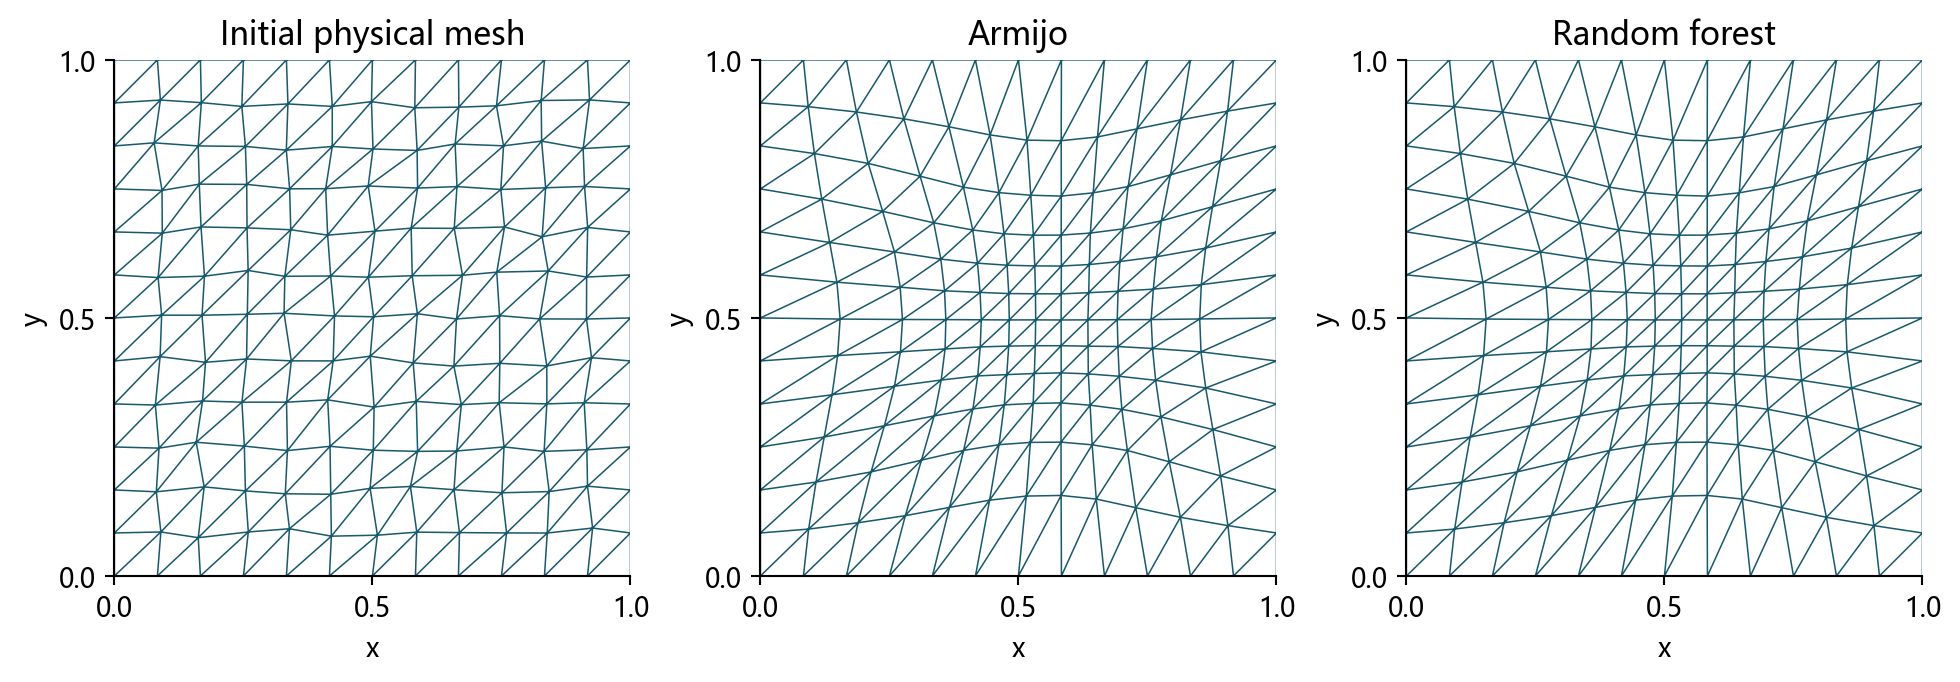
\includegraphics[width=\linewidth]{../figures/mesh_gaussian.png}\captionof{figure}{图2　高斯度量下的物理网格。相同初值经标准 Armijo 与随机森林策略优化，均在中心附近形成较密网格。}\end{center}

展示实例的度量中心约为 $(0.5633,0.4930)$。以该中心为圆心、半径0.2的圆内，初始节点数18，随机森林结果为39。局部集中来自给定度量和能量最小化，不能归因于森林预测本身；标准 Armijo 也获得几乎相同的网格。圆内计数仅作几何描述，不代表PDE误差降低。


\subsection*{3.4 算例三：光滑各向异性度量}

\begin{center}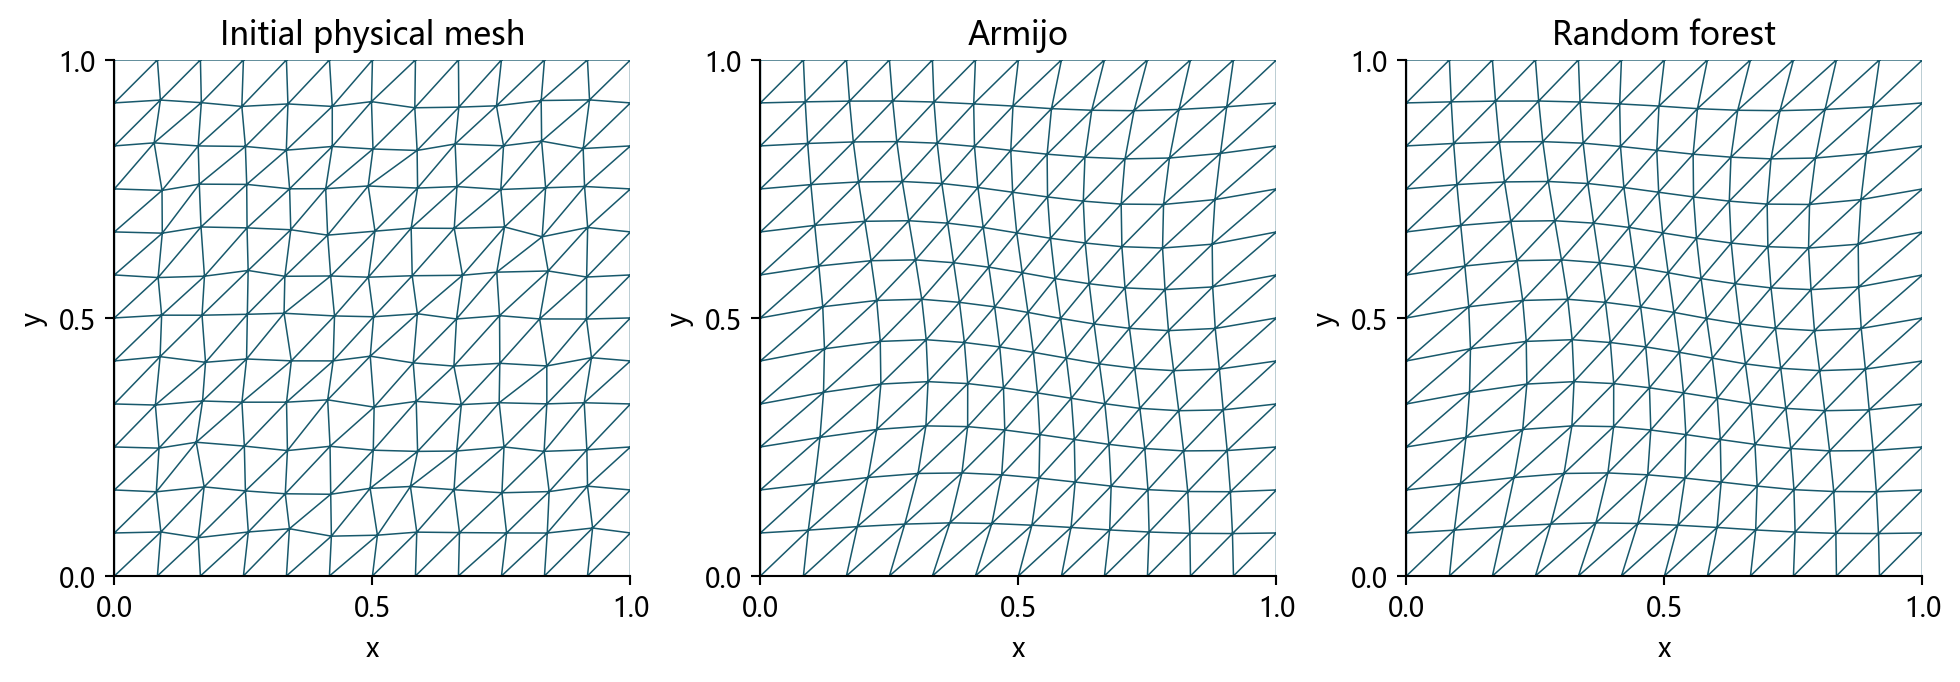
\includegraphics[width=\linewidth]{../figures/mesh_anisotropic.png}\captionof{figure}{图3　各向异性度量下的物理网格。固定方向与局部强度变化共同导致定向变形，四周边界保持固定。}\end{center}

本例在平滑权重上增加秩一方向项，观察局部网格的方向响应。中心圆内节点数从18变为25。用单元边矩阵的奇异值比作描述时，全域平均由2.662变为2.651：该指标受三角形顶点编号和原始剖分影响，不能将视觉拉伸直接解释为整体质量改善。这里更直接的证据是单元位置、朝向和能量的实际变化。三个展示实例均预先采用测试种子100，完整九个测试实例全部保留。


\newpage

\subsection*{3.5 四种方法的共同精度比较}

表2　三次独立测试实例的算术平均；所有行均3/3收敛，固定步长为0.05


\begin{center}\small\resizebox{\linewidth}{!}{\begin{tabular}{lllllll}\toprule
算例 & 方法 & 迭代数 & 能量评价 & 回溯数 & 时间/s & 最终能量 \\
\midrule
均匀度量 & 固定步长 & 238.0 & 239.0 & 0.0 & 0.566 & 2.00000001 \\
均匀度量 & Armijo & 100.0 & 382.0 & 299.7 & 0.301 & 2.00000001 \\
均匀度量 & 热启动 & 155.0 & 158.0 & 4.0 & 0.341 & 2.00000001 \\
均匀度量 & 随机森林 & 149.7 & 153.0 & 2.3 & 1.016 & 2.00000001 \\
局部高斯度量 & 固定步长 & 818.7 & 819.7 & 0.0 & 2.573 & 1.20041767 \\
局部高斯度量 & Armijo & 270.0 & 972.7 & 736.0 & 0.969 & 1.20041766 \\
局部高斯度量 & 热启动 & 325.0 & 327.0 & 3.0 & 1.143 & 1.20041767 \\
局部高斯度量 & 随机森林 & 274.3 & 298.0 & 22.7 & 2.517 & 1.20041766 \\
各向异性度量 & 固定步长 & 547.3 & 548.3 & 0.0 & 1.563 & 1.60743644 \\
各向异性度量 & Armijo & 228.0 & 891.0 & 677.0 & 0.736 & 1.60743643 \\
各向异性度量 & 热启动 & 217.7 & 219.7 & 3.0 & 0.610 & 1.60743644 \\
各向异性度量 & 随机森林 & 215.3 & 240.0 & 23.7 & 1.710 & 1.60743643 \\
\bottomrule\end{tabular}}\end{center}


\begin{center}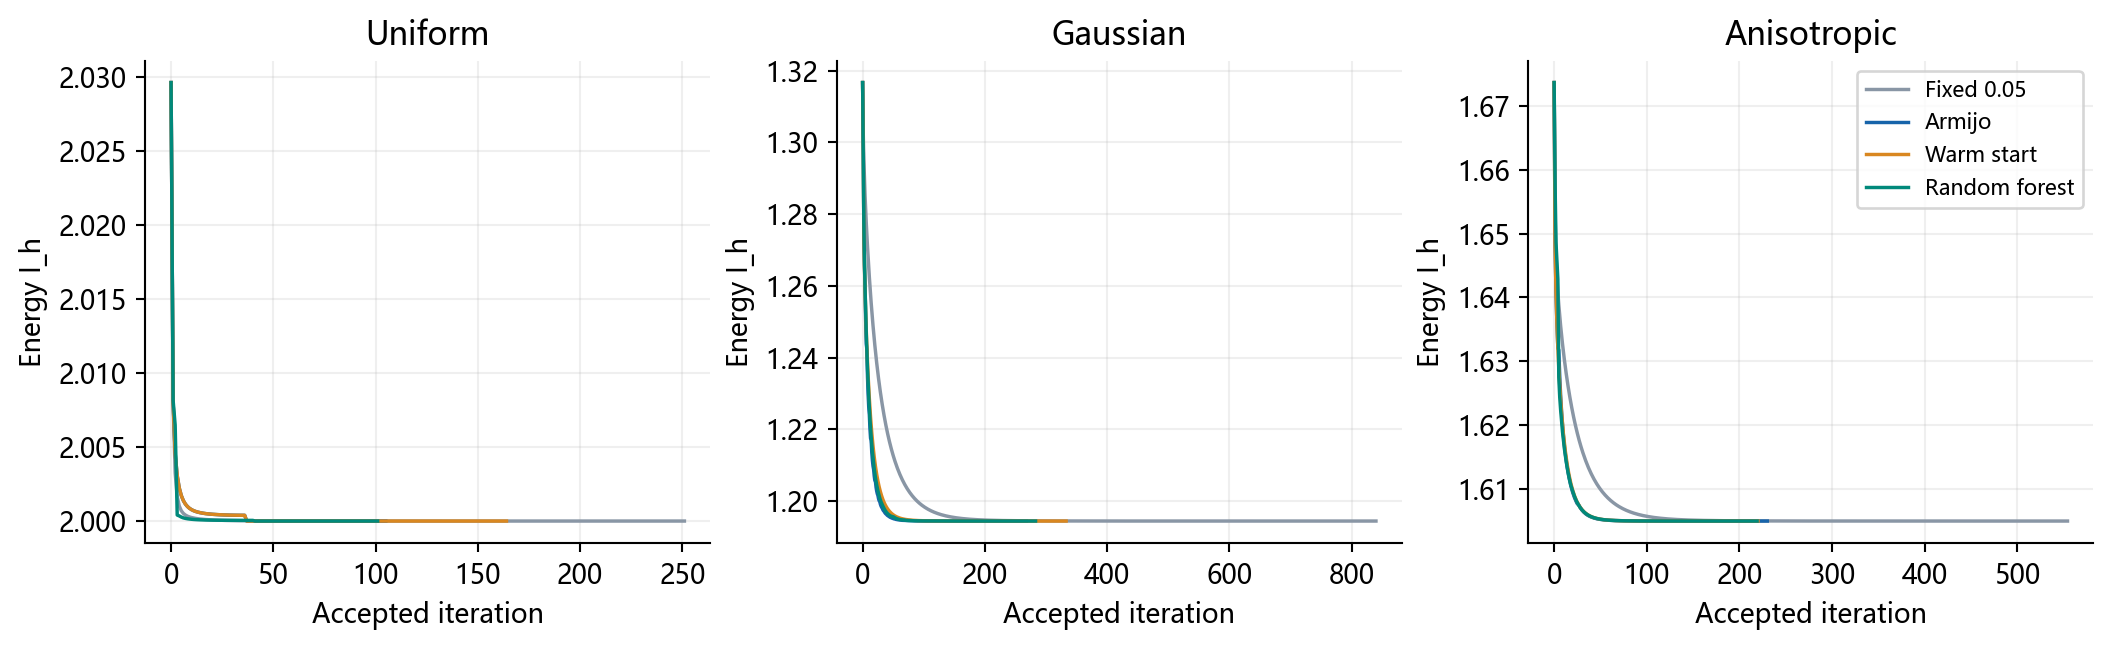
\includegraphics[width=\linewidth]{../figures/energy.png}\captionof{figure}{图4　三个展示实例的离散能量随接受迭代数变化；各面板使用各自能量尺度。}\end{center}

三十六次运行全部达到共同梯度阈值，最终物理网格的翻转单元总数为 0，所有测试运行最终最小物理定向面积的最小值为 1.213e-03。同一实例不同方法的最终能量非常接近，表中小差异来自停止阈值及数值路径。相对能量降幅、最终梯度范数、计算与物理最小面积均在原始结果表中逐次保存。


森林在均匀、高斯和各向异性算例分别平均执行 2.3、22.7 和 23.7 次回溯。热启动仅在必要时缩小历史步长，成本很低，但不能主动增大步长，可能增加迭代数。固定步长虽无回溯，其收敛过程需要较多迭代，因此评价次数最少或回溯最少都不足以单独判断方法优劣。


\newpage

\section*{4 结果讨论}

\subsection*{4.1 评价节省与时间成本}

\begin{center}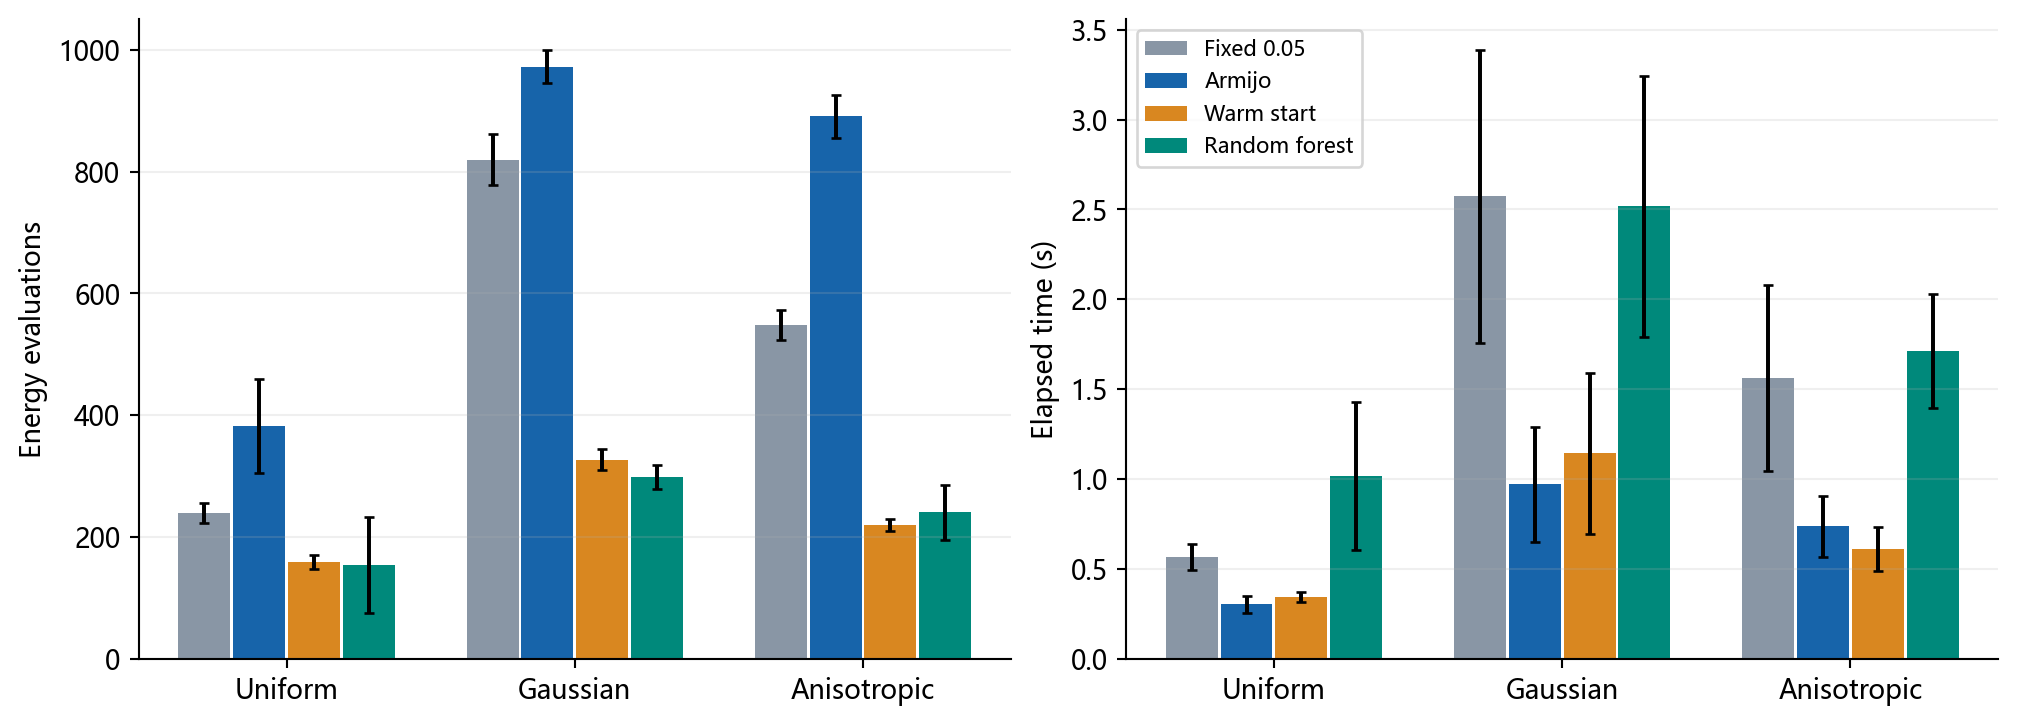
\includegraphics[width=\linewidth]{../figures/cost.png}\captionof{figure}{图5　能量评价次数及总耗时，误差棒为三个独立实例的样本标准差。}\end{center}

随机森林相对固定初值 Armijo 的能量评价次数分别减少 59.9\%、69.4\% 和 73.1\%，但总耗时分别为其 3.38、2.60 和 2.33 倍。在本次小规模网格上，学习初始步长未带来端到端加速。 森林在三个算例上也均慢于热启动。其特征提取与推理占森林求解总耗时的 64.8\%。对288个单元，NumPy 的能量计算较便宜，逐步调用森林的固定开销超过节省的候选检查成本。


表3　总耗时的均值与样本标准差，单位：秒


\begin{center}\small\resizebox{\linewidth}{!}{\begin{tabular}{lllll}\toprule
算例 & 固定步长/s & Armijo/s & 热启动/s & 随机森林/s \\
\midrule
均匀度量 & 0.566 ± 0.073 & 0.301 ± 0.046 & 0.341 ± 0.026 & 1.016 ± 0.410 \\
局部高斯度量 & 2.573 ± 0.815 & 0.969 ± 0.321 & 1.143 ± 0.449 & 2.517 ± 0.728 \\
各向异性度量 & 1.563 ± 0.519 & 0.736 ± 0.170 & 0.610 ± 0.125 & 1.710 ± 0.317 \\
\bottomrule\end{tabular}}\end{center}


\subsection*{4.2 模仿标签与预测质量}

\begin{center}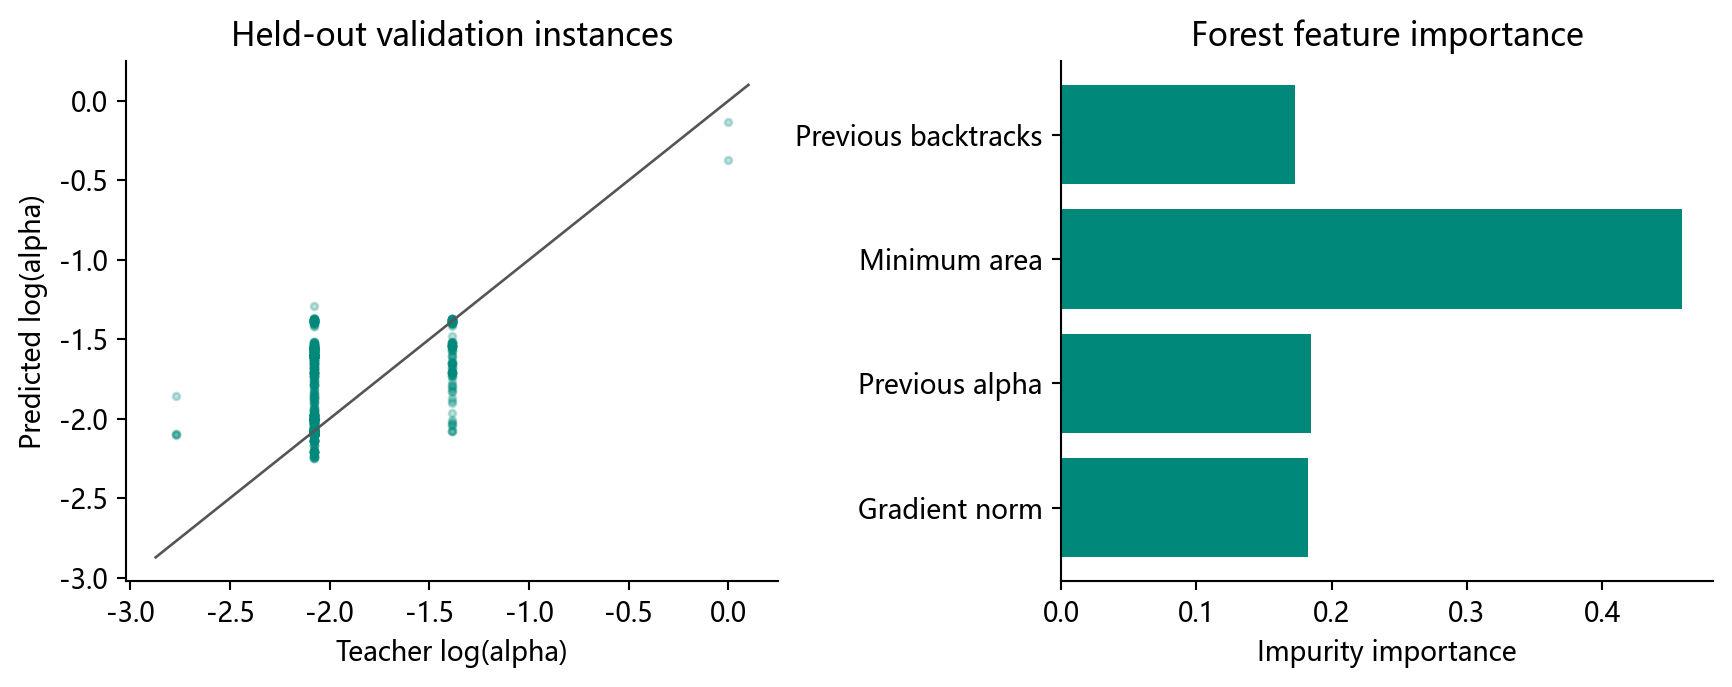
\includegraphics[width=\linewidth]{../figures/model.png}\captionof{figure}{图6　独立验证实例的对数步长预测及森林的特征重要性；重要性是模型内的杂质下降统计。}\end{center}

验证集对数步长 MAE 为 0.1848，$R^2=-0.5623$；直接使用前一步对数步长的 MAE 为 0.1638。负 $R^2$ 表示预测弱于使用验证标签均值的常数预测。训练标签标准差为 0.2387，森林未建立强预测优势。标签来自固定初值及二分回溯，是教师算法的离散选择，既不是最大可行步长，也不是耗时最优标签。


\newpage

\subsection*{4.3 局限}

本实验只有三个度量家族，每类三个未见实例；训练与测试来自相同参数区间，不能推断跨家族或大规模泛化。森林在自身优化轨迹上访问的状态可能偏离教师数据，实例隔离并不能消除这种分布变化。当前报告为一次完整批量运行；误差棒表示实例间差异，并非同一实例多次计时的测量置信区间。运行时间还受本机后台负载影响，稳定可复核的指标是配置、轨迹、评价计数和停止条件。


所有比较使用同一个冻结物理网格上的二次能量，没有外层度量更新；固定边界限制了可达到的变形。定向面积检查是每个离散候选的实际验收条件，不是任意输入下的非退化定理。这里比较简化显式梯度法的线搜索，不是对2015年论文中 ode15s 求解器的直接加速，也没有实现[2]的循环模型或[3]的CFD流程。


教师数据生成耗时 21.168 秒，模型拟合耗时 0.430 秒；二者单列，不并入测试求解时间。由于本次推理阶段本身没有时间收益，当前测量不存在可摊平训练成本的正复用次数。是否能在更大规模或更昂贵的能量上获益，需要另外的对照实验，而不是由评价次数减少推断。


\section*{5 结论}

本课程设计完成了一条可复现的轻量机器学习数值实验流程：复用解析能量与梯度，生成传统轨迹，按完整实例训练与验证随机森林，并在三个二维算例上与三种传统策略比较。全部测试运行达到同一梯度标准且网格保持正定向；高斯度量产生明确的局部集中，说明优化与映射流程在这些实例上工作正常。


实验支持两个结论：第一，安全层允许预测步长参与迭代而保持本批次接受步的充分下降和网格合法性；第二，在本次小网格与实现条件下，节省能量评价不足以补偿随机森林开销。实际使用应优先选择简单 Armijo 或热启动，并根据求解总成本判断学习模块是否值得加入。


\section*{参考文献}

[1] Huang W., Kamenski L., Russell R. D. A comparative numerical study of meshing functionals for variational mesh adaptation. Journal of Mathematics Study, 2015, 48(2): 168–186. DOI: 10.4208/jms.v48n2.15.04. \href{https://arxiv.org/abs/1503.04709}{预印本}。


[2] Kamandi A. Learning the initial step size and backtracking reduction factor for the Armijo line search. Journal of Mathematical Modeling, 2026, Articles in Press, Corrected Proof，2026-08-18 在线发表. DOI: 10.22124/jmm.2026.33801.3107. \href{https://jmm.guilan.ac.ir/article\_9844.html}{期刊页面}。


[3] Wu T., Liu X., An W., Huang Z., Lyu H. A mesh optimization method using machine learning technique and variational mesh adaptation. Chinese Journal of Aeronautics, 2022, 35(3): 27–41. DOI: 10.1016/j.cja.2021.05.018. \href{https://www.sciopen.com/article/10.1016/j.cja.2021.05.018}{期刊页面}。


\textbf{数据与复现：} 项目包含完整配置、训练划分、逐步轨迹、测试结果表、网格坐标、模型和绘图代码。运行 \texttt{python scripts/reproduce.py} 可重建实验、图表、报告及汇报页；报告数值由结果文件自动读取，全部运行记录均纳入统计。

\end{document}